\section{Initial results}
\label{sec:eval}

% \heidi{I do think the paper would benefit from some results, either from a component of 2P-Set or PBFT as discussed even if component is very limited. The results really help to motivate the rest of the paper}
% \heidi{One paper you might want to look at (also from PaPoc: https://martin.kleppmann.com/papers/bft-crdt-papoc22.pdf}

\begin{figure}[t]
    \centering
    \begin{tikzpicture}[
arrows={-Triangle[scale=0.75]},
very thick,
draw=black!40,
node distance=12.5mm,
point/.style={coordinate, text=black, very thick},
placeholder/.style={rectangle, text=black, very thick},
client/.style={circle, draw=black!0, very thick, minimum size=3.5mm},
pics/legend entry/.style={code={%   
        \draw[-, thick] 
        (-0.25,0.2) -- (0.25,0.2);}}],
]
%Nodes
\node[client]        (leftclient)                           {};
% \node[placeholder]        (leftclientplaceholder)       [below=of leftclient] {};

\node[placeholder]        (l1lleftendpoint)       [below=4.5mm of leftclient] {};
\node[placeholder]        (l1plleftendpoint)       [below=0mm of l1lleftendpoint] {};
\node[placeholder]        (l1ppleftendpoint)       [below=0mm of l1plleftendpoint] {};
\node[placeholder]        (l1pleftendpoint)       [below=0mm of l1ppleftendpoint] {};
\node[placeholder]        (l1cleftendpoint)       [below=0mm of l1pleftendpoint] {};
\node[placeholder]        (l2lleftendpoint)       [below=4.5mm of l1cleftendpoint] {};
\node[placeholder]        (l2plleftendpoint)       [below=0mm of l2lleftendpoint] {};
\node[placeholder]        (l2ppleftendpoint)       [below=0mm of l2plleftendpoint] {};
\node[placeholder]        (l2pleftendpoint)       [below=0mm of l2ppleftendpoint] {};
\node[placeholder]        (l2cleftendpoint)       [below=0mm of l2pleftendpoint] {};

\node[placeholder]        (l3lleftendpoint)       [below=4.5mm of l2cleftendpoint] {};
\node[placeholder]        (l3plleftendpoint)       [below=0mm of l3lleftendpoint] {};
\node[placeholder]        (l3ppleftendpoint)       [below=0mm of l3plleftendpoint] {};
\node[placeholder]        (l3pleftendpoint)       [below=0mm of l3ppleftendpoint] {};
\node[placeholder]        (l3cleftendpoint)       [below=0mm of l3pleftendpoint] {};
\node[placeholder]        (l4lleftendpoint)       [below=4.5mm of l3cleftendpoint] {};
\node[placeholder]        (l4plleftendpoint)       [below=0mm of l4lleftendpoint] {};
\node[placeholder]        (l4ppleftendpoint)       [below=0mm of l4plleftendpoint] {};
\node[placeholder]        (l4pleftendpoint)       [below=0mm of l4ppleftendpoint] {};
\node[placeholder]        (l4cleftendpoint)       [below=0mm of l4pleftendpoint] {};

\node[point]        (t1l1l)       [right=of l1lleftendpoint] {};
\node[point]        (t1l1pl)       [right=of l1plleftendpoint] {};
\node[point]        (t1l1pp)       [right=of l1ppleftendpoint] {};
\node[point]        (t1l1p)       [right=of l1pleftendpoint] {};
\node[point]        (t1l1c)       [right=of l1cleftendpoint] {};
\node[point]        (t1l2l)       [right=of l2lleftendpoint] {};
\node[point]        (t1l2pl)       [right=of l2plleftendpoint] {};
\node[point]        (t1l2pp)       [right=of l2ppleftendpoint] {};
\node[point]        (t1l2p)       [right=of l2pleftendpoint] {};
\node[point]        (t1l2c)       [right=of l2cleftendpoint] {};

\node[point]        (t1l3l)       [right=of l3lleftendpoint] {};
\node[point]        (t1l3pl)       [right=of l3plleftendpoint] {};
\node[point]        (t1l3pp)       [right=of l3ppleftendpoint] {};
\node[point]        (t1l3p)       [right=of l3pleftendpoint] {};
\node[point]        (t1l3c)       [right=of l3cleftendpoint] {};
\node[point]        (t1l4l)       [right=of l4lleftendpoint] {};
\node[point]        (t1l4pl)       [right=of l4plleftendpoint] {};
\node[point]        (t1l4pp)       [right=of l4ppleftendpoint] {};
\node[point]        (t1l4p)       [right=of l4pleftendpoint] {};
\node[point]        (t1l4c)       [right=of l4cleftendpoint] {};

\node[point]        (t2l1l)       [right=of t1l1l] {};
\node[point]        (t2l1pl)       [right=of t1l1pl] {};
\node[point]        (t2l1pp)       [right=of t1l1pp] {};
\node[point]        (t2l1p)       [right=of t1l1p] {};
\node[point]        (t2l1c)       [right=of t1l1c] {};
\node[point]        (t2l2l)       [right=of t1l2l] {};
\node[point]        (t2l2pl)       [right=of t1l2pl] {};
\node[point]        (t2l2pp)       [right=of t1l2pp] {};
\node[point]        (t2l2p)       [right=of t1l2p] {};
\node[point]        (t2l2c)       [right=of t1l2c] {};

\node[point]        (t2l3l)       [right=of t1l3l] {};
\node[point]        (t2l3pl)       [right=of t1l3pl] {};
\node[point]        (t2l3pp)       [right=of t1l3pp] {};
\node[point]        (t2l3p)       [right=of t1l3p] {};
\node[point]        (t2l3c)       [right=of t1l3c] {};
\node[point]        (t2l4l)       [right=of t1l4l] {};
\node[point]        (t2l4pl)       [right=of t1l4pl] {};
\node[point]        (t2l4pp)       [right=of t1l4pp] {};
\node[point]        (t2l4p)       [right=of t1l4p] {};
\node[point]        (t2l4c)       [right=of t1l4c] {};

\node[point]        (t3l1l)       [right=of t2l1l] {};
\node[point]        (t3l1pl)       [right=of t2l1pl] {};
\node[point]        (t3l1pp)       [right=of t2l1pp] {};
\node[point]        (t3l1p)       [right=of t2l1p] {};
\node[point]        (t3l1c)       [right=of t2l1c] {};
\node[point]        (t3l2l)       [right=of t2l2l] {};
\node[point]        (t3l2pl)       [right=of t2l2pl] {};
\node[point]        (t3l2pp)       [right=of t2l2pp] {};
\node[point]        (t3l2p)       [right=of t2l2p] {};
\node[point]        (t3l2c)       [right=of t2l2c] {};

\node[point]        (t3l3l)       [right=of t2l3l] {};
\node[point]        (t3l3pl)       [right=of t2l3pl] {};
\node[point]        (t3l3pp)       [right=of t2l3pp] {};
\node[point]        (t3l3p)       [right=of t2l3p] {};
\node[point]        (t3l3c)       [right=of t2l3c] {};
\node[point]        (t3l4l)       [right=of t2l4l] {};
\node[point]        (t3l4pl)       [right=of t2l4pl] {};
\node[point]        (t3l4pp)       [right=of t2l4pp] {};
\node[point]        (t3l4p)       [right=of t2l4p] {};
\node[point]        (t3l4c)       [right=of t2l4c] {};

\node[point]        (t4l1l)       [right=of t3l1l] {};
\node[point]        (t4l1pl)       [right=of t3l1pl] {};
\node[point]        (t4l1pp)       [right=of t3l1pp] {};
\node[point]        (t4l1p)       [right=of t3l1p] {};
\node[point]        (t4l1c)       [right=of t3l1c] {};
\node[point]        (t4l2l)       [right=of t3l2l] {};
\node[point]        (t4l2pl)       [right=of t3l2pl] {};
\node[point]        (t4l2pp)       [right=of t3l2pp] {};
\node[point]        (t4l2p)       [right=of t3l2p] {};
\node[point]        (t4l2c)       [right=of t3l2c] {};

\node[point]        (t4l3l)       [right=of t3l3l] {};
\node[point]        (t4l3pl)       [right=of t3l3pl] {};
\node[point]        (t4l3pp)       [right=of t3l3pp] {};
\node[point]        (t4l3p)       [right=of t3l3p] {};
\node[point]        (t4l3c)       [right=of t3l3c] {};
\node[point]        (t4l4l)       [right=of t3l4l] {};
\node[point]        (t4l4pl)       [right=of t3l4pl] {};
\node[point]        (t4l4pp)       [right=of t3l4pp] {};
\node[point]        (t4l4p)       [right=of t3l4p] {};
\node[point]        (t4l4c)       [right=of t3l4c] {};

\node[point]        (t5l1l)       [right=of t4l1l] {};
\node[point]        (t5l1pl)       [right=of t4l1pl] {};
\node[point]        (t5l1pp)       [right=of t4l1pp] {};
\node[point]        (t5l1p)       [right=of t4l1p] {};
\node[point]        (t5l1c)       [right=of t4l1c] {};
\node[point]        (t5l2l)       [right=of t4l2l] {};
\node[point]        (t5l2pl)       [right=of t4l2pl] {};
\node[point]        (t5l2pp)       [right=of t4l2pp] {};
\node[point]        (t5l2p)       [right=of t4l2p] {};
\node[point]        (t5l2c)       [right=of t4l2c] {};

\node[point]        (t5l3l)       [right=of t4l3l] {};
\node[point]        (t5l3pl)       [right=of t4l3pl] {};
\node[point]        (t5l3pp)       [right=of t4l3pp] {};
\node[point]        (t5l3p)       [right=of t4l3p] {};
\node[point]        (t5l3c)       [right=of t4l3c] {};
\node[point]        (t5l4l)       [right=of t4l4l] {};
\node[point]        (t5l4pl)       [right=of t4l4pl] {};
\node[point]        (t5l4pp)       [right=of t4l4pp] {};
\node[point]        (t5l4p)       [right=of t4l4p] {};
\node[point]        (t5l4c)       [right=of t4l4c] {};

\node[placeholder]        (l1lrightendpoint)       [right=of t5l1l] {};
\node[placeholder]        (l1plrightendpoint)       [right=of t5l1pl] {};
\node[placeholder]        (l1pprightendpoint)       [right=of t5l1pp] {};
\node[placeholder]        (l1prightendpoint)       [right=of t5l1p] {};
\node[placeholder]        (l1crightendpoint)       [right=of t5l1c] {};
\node[placeholder]        (l2lrightendpoint)       [right=of t5l2l] {};
\node[placeholder]        (l2plrightendpoint)       [right=of t5l2pl] {};
\node[placeholder]        (l2pprightendpoint)       [right=of t5l2pp] {};
\node[placeholder]        (l2prightendpoint)       [right=of t5l2p] {};
\node[placeholder]        (l2crightendpoint)       [right=of t5l2c] {};

\node[placeholder]        (l3lrightendpoint)       [right=of t5l3l] {};
\node[placeholder]        (l3plrightendpoint)       [right=of t5l3pl] {};
\node[placeholder]        (l3pprightendpoint)       [right=of t5l3pp] {};
\node[placeholder]        (l3prightendpoint)       [right=of t5l3p] {};
\node[placeholder]        (l3crightendpoint)       [right=of t5l3c] {};
\node[placeholder]        (l4lrightendpoint)       [right=of t5l4l] {};
\node[placeholder]        (l4plrightendpoint)       [right=of t5l4pl] {};
\node[placeholder]        (l4pprightendpoint)       [right=of t5l4pp] {};
\node[placeholder]        (l4prightendpoint)       [right=of t5l4p] {};
\node[placeholder]        (l4crightendpoint)       [right=of t5l4c] {};

% \node[placeholder]        (rightclientplaceholder)       [right=of t5l1l] {};
\node[client]        (rightclient)       [above=4.5mm of l1lrightendpoint] {};

% \node[placeholder]        (t1label)       [above=4.5mm of t1l1l] [text depth=0pt]{$t_1$};
% \node[placeholder]        (t2label)       [above=4.5mm of t2l1l] [text depth=0pt]{$t_2$};
% \node[placeholder]        (t3label)       [above=4.5mm of t3l1l] [text depth=0pt]{$t_3$};
% \node[placeholder]        (t4label)       [above=4.5mm of t4l1l] [text depth=0pt]{$t_4$};
% \node[placeholder]        (t5label)       [above=4.5mm of t5l1l] [text depth=0pt]{$t_5$};

\node[placeholder, above=9mm of $(l1lleftendpoint)!0.5!(t1l1l)$] (reqlabel) [text depth=0pt]{\tiny request};
\node[placeholder, above=9mm of $(t1l1l)!0.5!(t2l1l)$] (seqlabel) [text depth=0pt]{\tiny sequencing};
\node[placeholder, above=9mm of $(t2l1l)!0.5!(t3l1l)$] (pplabel) [text depth=0pt]{\tiny pre-prepare};
\node[placeholder, above=9mm of $(t3l1l)!0.5!(t4l1l)$] (plabel) [text depth=0pt]{\tiny prepare};
\node[placeholder, above=9mm of $(t4l1l)!0.5!(t5l1l)$] (comlabel) [text depth=0pt]{\tiny commit};
\node[placeholder, above=9mm of $(t5l1l)!0.5!(l1lrightendpoint)$] (repllabel) [text depth=0pt]{\tiny reply};

% \node[placeholder, above=0mm of $reqlabel:!0.5!seqlabel$] (b1top) {};
% \node[placeholder, above=0mm of $seqlabel:!0.5!pplabel$] (b2top) {};
% \node[placeholder, above=0mm of $pplabel:!0.5!plabel$] (b3top) {};
% \node[placeholder, above=0mm of $plabel:!0.5!comlabel$] (b4top) {};
% \node[placeholder, above=0mm of $comlabel:!0.5!replabel$] (b5top) {};

% \node[placeholder, below=40mm of $reqlabel:!0.5!seqlabel$] (b1bot) {};
% \node[placeholder, below=40mm of $seqlabel:!0.5!pplabel$] (b2bot) {};
% \node[placeholder, below=40mm of $pplabel:!0.5!plabel$] (b3bot) {};
% \node[placeholder, below=40mm of $plabel:!0.5!comlabel$] (b4bot) {};
% \node[placeholder, below=40mm of $comlabel:!0.5!replabel$] (b5bot) {};

\node[placeholder]        (l1label)       [left=1.5mm of l1ppleftendpoint.south] {$r_1$};
\node[placeholder]        (l2label)       [left=1.5mm of l2ppleftendpoint.south] {$r_2$};
\node[placeholder]        (l3label)       [left=1.5mm of l3ppleftendpoint.south] {$r_3$};
\node[placeholder]        (l4label)       [left=1.5mm of l4ppleftendpoint.south] {$r_4$};

\matrix [draw, above] at (3.5,-8.5) {
 \pic[blue!40]{legend entry}; &  \node[font=\tiny,text depth=0pt] {leader}; & \pic[blue!40, densely dash dot dot]{legend entry}; &  \node[font=\tiny,text depth=0pt] {proxy leader}; & \pic[red, dashed]{legend entry}; &  \node[font=\tiny,text depth=0pt] {pre-preparer}; & \pic[green!40!black, densely dotted]{legend entry}; &  \node[font=\tiny,text depth=0pt] {preparer}; & \pic[yellow!40!orange, dashdotted]{legend entry}; &  \node[font=\tiny,text depth=0pt] {committer}; \\
};

%Lines
\begin{pgfonlayer}{bg}
    \draw[-] (l1lleftendpoint) -- (l1lrightendpoint) [draw=blue!40, thick];
    \draw[-] (l1plleftendpoint) -- (l1plrightendpoint) [draw=blue!40, thick, densely dash dot dot];
    \draw[-] (l1ppleftendpoint) -- (l1pprightendpoint) [draw=red, dashed, thick];
    \draw[-] (l1pleftendpoint) -- (l1prightendpoint) [draw=green!40!black, densely dotted, thick];
    \draw[-] (l1cleftendpoint) -- (l1crightendpoint) [draw=yellow!40!orange, dashdotted, thick];
    \draw[-] (l2lleftendpoint) -- (l2lrightendpoint) [draw=blue!40, thick];
    \draw[-] (l2plleftendpoint) -- (l2plrightendpoint) [draw=blue!40, thick, densely dash dot dot];
    \draw[-] (l2ppleftendpoint) -- (l2pprightendpoint) [draw=red, dashed, thick];
    \draw[-] (l2pleftendpoint) -- (l2prightendpoint) [draw=green!40!black, densely dotted, thick];
    \draw[-] (l2cleftendpoint) -- (l2crightendpoint) [draw=yellow!40!orange, dashdotted, thick];
    \draw[-] (l3lleftendpoint) -- (l3lrightendpoint) [draw=blue!40, thick];
    \draw[-] (l3plleftendpoint) -- (l3plrightendpoint) [draw=blue!40, thick, densely dash dot dot];
    \draw[-] (l3ppleftendpoint) -- (l3pprightendpoint) [draw=red, dashed, thick];
    \draw[-] (l3pleftendpoint) -- (l3prightendpoint) [draw=green!40!black, densely dotted, thick];
    \draw[-] (l3cleftendpoint) -- (l3crightendpoint) [draw=yellow!40!orange, dashdotted, thick];
    \draw[-] (l4lleftendpoint) -- (l4lrightendpoint) [draw=blue!40, thick];
    \draw[-] (l4plleftendpoint) -- (l4plrightendpoint) [draw=blue!40, thick, densely dash dot dot];
    \draw[-] (l4ppleftendpoint) -- (l4pprightendpoint) [draw=red, dashed, thick];
    \draw[-] (l4pleftendpoint) -- (l4prightendpoint) [draw=green!40!black, densely dotted, thick];
    \draw[-] (l4cleftendpoint) -- (l4crightendpoint) [draw=yellow!40!orange, dashdotted, thick];
\end{pgfonlayer}

\draw[arrows={-Triangle[scale=0.75]}] (leftclient) -- (t1l1l) [very thick, draw=black];

% \draw[arrows={-Triangle[scale=0.75]}] (t1l1l) -- (t2l1pl) [very thick, draw=black];

\draw[arrows={-Triangle[scale=0.75]}] (t2l1pl) -- (t3l1pp);
% \draw[arrows={-Triangle[scale=0.75]}] (t2l1pl) -- (t3l2pp) [very thick, draw=black];
\draw[arrows={-Triangle[scale=0.75]}] (t2l1pl) -- (t3l3pp);
\draw[arrows={-Triangle[scale=0.75]}] (t2l1pl) -- (t3l4pp);

\draw[arrows={-Triangle[scale=0.75]}] (t3l1pp) -- (t4l1c);
% \draw[arrows={-Triangle[scale=0.75]}] (t3l2pp) -- (t4l2c) [very thick, draw=black];
\draw[arrows={-Triangle[scale=0.75]}] (t3l3pp) -- (t4l3c);
\draw[arrows={-Triangle[scale=0.75]}] (t3l4pp) -- (t4l4c);

\draw[arrows={-Triangle[scale=0.75]}] (t3l1pp) -- (t4l1p);
\draw[arrows={-Triangle[scale=0.75]}] (t3l1pp) -- (t4l2p);
\draw[arrows={-Triangle[scale=0.75]}] (t3l1pp) -- (t4l3p);
\draw[arrows={-Triangle[scale=0.75]}] (t3l1pp) -- (t4l4p);
% \draw[arrows={-Triangle[scale=0.75]}] (t3l2pp) -- (t4l1p) [very thick, draw=black];
% \draw[arrows={-Triangle[scale=0.75]}] (t3l2pp) -- (t4l2p) [very thick, draw=black];
% \draw[arrows={-Triangle[scale=0.75]}] (t3l2pp) -- (t4l3p) [very thick, draw=black];
% \draw[arrows={-Triangle[scale=0.75]}] (t3l2pp) -- (t4l4p) [very thick, draw=black];
\draw[arrows={-Triangle[scale=0.75]}] (t3l3pp) -- (t4l1p);
\draw[arrows={-Triangle[scale=0.75]}] (t3l3pp) -- (t4l2p);
\draw[arrows={-Triangle[scale=0.75]}] (t3l3pp) -- (t4l3p);
\draw[arrows={-Triangle[scale=0.75]}] (t3l3pp) -- (t4l4p);
\draw[arrows={-Triangle[scale=0.75]}] (t3l4pp) -- (t4l1p);
\draw[arrows={-Triangle[scale=0.75]}] (t3l4pp) -- (t4l2p);
\draw[arrows={-Triangle[scale=0.75]}] (t3l4pp) -- (t4l3p);
\draw[arrows={-Triangle[scale=0.75]}] (t3l4pp) -- (t4l4p);

\draw[arrows={-Triangle[scale=0.75]}] (t4l1p) -- (t5l1c);
\draw[arrows={-Triangle[scale=0.75]}] (t4l1p) -- (t5l2c);
\draw[arrows={-Triangle[scale=0.75]}] (t4l1p) -- (t5l3c);
\draw[arrows={-Triangle[scale=0.75]}] (t4l1p) -- (t5l4c);
% \draw[arrows={-Triangle[scale=0.75]}] (t4l2p) -- (t5l1c) [very thick, draw=black];
% \draw[arrows={-Triangle[scale=0.75]}] (t4l2p) -- (t5l2c) [very thick, draw=black];
% \draw[arrows={-Triangle[scale=0.75]}] (t4l2p) -- (t5l3c) [very thick, draw=black];
% \draw[arrows={-Triangle[scale=0.75]}] (t4l2p) -- (t5l4c) [very thick, draw=black];
\draw[arrows={-Triangle[scale=0.75]}] (t4l3p) -- (t5l1c);
\draw[arrows={-Triangle[scale=0.75]}] (t4l3p) -- (t5l2c);
\draw[arrows={-Triangle[scale=0.75]}] (t4l3p) -- (t5l3c);
\draw[arrows={-Triangle[scale=0.75]}] (t4l3p) -- (t5l4c);
\draw[arrows={-Triangle[scale=0.75]}] (t4l4p) -- (t5l1c);
\draw[arrows={-Triangle[scale=0.75]}] (t4l4p) -- (t5l2c);
\draw[arrows={-Triangle[scale=0.75]}] (t4l4p) -- (t5l3c);
\draw[arrows={-Triangle[scale=0.75]}] (t4l4p) -- (t5l4c);

\draw[arrows={-Triangle[scale=0.75]}] (t5l1c) -- (rightclient);
% \draw[arrows={-Triangle[scale=0.75]}] (t5l2c) -- (rightclient) [very thick, draw=black];
\draw[arrows={-Triangle[scale=0.75]}] (t5l3c) -- (rightclient);
\draw[arrows={-Triangle[scale=0.75]}] (t5l4c) -- (rightclient);

\draw[arrows={-Triangle[scale=0.75]}] (t1l1l) -- (t2l1pl) [very thick, draw=black];
\draw[arrows={-Triangle[scale=0.75]}] (t2l1pl) -- (t3l2pp) [very thick, draw=black];
\draw[arrows={-Triangle[scale=0.75]}] (t3l2pp) -- (t4l2c) [very thick, draw=black];
\draw[arrows={-Triangle[scale=0.75]}] (t3l2pp) -- (t4l1p) [very thick, draw=black];
\draw[arrows={-Triangle[scale=0.75]}] (t3l2pp) -- (t4l2p) [very thick, draw=black];
\draw[arrows={-Triangle[scale=0.75]}] (t3l2pp) -- (t4l3p) [very thick, draw=black];
\draw[arrows={-Triangle[scale=0.75]}] (t3l2pp) -- (t4l4p) [very thick, draw=black];
\draw[arrows={-Triangle[scale=0.75]}] (t4l2p) -- (t5l1c) [very thick, draw=black];
\draw[arrows={-Triangle[scale=0.75]}] (t4l2p) -- (t5l2c) [very thick, draw=black];
\draw[arrows={-Triangle[scale=0.75]}] (t4l2p) -- (t5l3c) [very thick, draw=black];
\draw[arrows={-Triangle[scale=0.75]}] (t4l2p) -- (t5l4c) [very thick, draw=black];
\draw[arrows={-Triangle[scale=0.75]}] (t5l2c) -- (rightclient) [very thick, draw=black];

\end{tikzpicture}
     \caption{The critical path of \ScalablePBFT{}, with the message path through $r_2$ bolded. $r_1$ is the primary.}
    \label{fig:decoupledPBFT}
\end{figure}

We evaluate the efficacy of our rule-driven rewrites by manually applying them to scale the critical path of PBFT~\cite{pbft}.
Our experimental scripts and setup can be found at \url{https://github.com/rithvikp/autocomp}.

\david{Experimental setup.}
Our evaluation mirrors the evaluation from \sigmodpaper{}
PBFT is implemented in Dedalus~\cite{dedalus} and compiled to Hydroflow~\cite{hydroflow}, a Rust dataflow runtime for distributed systems.
We use SHA-256 to generate MACs and digests instead of md5 (as described in PBFT) due to known exploits on md5~\cite{breakMD5}.
We deploy on GCP using n2-standard-4 machines with 4 vCPUs, 16 GB RAM, and 10 Gbps network bandwidth.
Throughput and latency are measured over one minute runs after 30 seconds of warmup.
Clients send 16 byte, unbatched, commands in a closed loop.
The state machines, clients, and protocol nodes are all run on separate machines.
Performance is measured with an increasing set of clients until throughput saturates, averaging across 3 runs with standard deviations in shaded regions.

\david{What we mean by implementing PBFT.}
We will refer to the unoptimized implementation of PBFT as \BasePBFT{} and the rewritten implementation as \ScalablePBFT{}.
Both implementations only include the critical path and assume that there is no view-change and no checkpoints.
Our deployments tolerate $f=1$ failures.
\Cref{fig:throughput} compares the resulting throughput-latency graph from both implementations.

\begin{figure}[t]
    \centering
    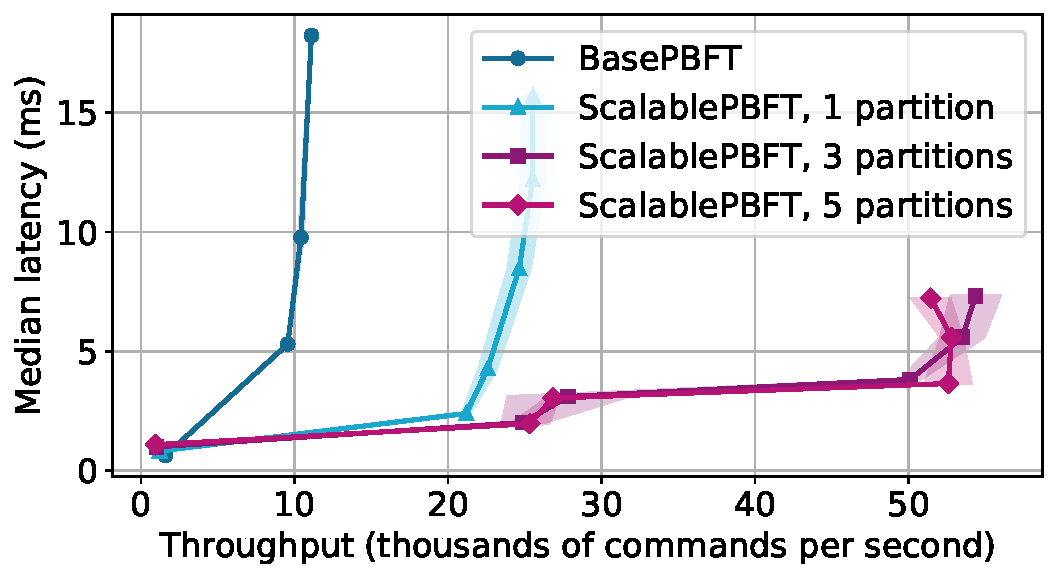
\includegraphics[width=0.6\linewidth]{assets/pbft_lt.pdf}
    \caption{Throughput/latency comparison of PBFT before and after rewrites.}
    \label{fig:throughput}
\end{figure}

\textbf{\BasePBFT{}.}
The base deployment contains $3f+1 = 4$ nodes.
Clients send messages to a pre-elected primary, which sequences the command and broadcasts \textsc{PrePrepare}s (including both the command and its signed digest).
Replicas that receive \textsc{PrePrepare}s broadcast \textsc{Prepare} (now only including the command's digest).
Replicas that receive $2f+1$ \textsc{Prepare}s broadcast a \textsc{Commit}, as seen in \Cref{alg:running-example}.
Replicas that receive $2f+1$ \textsc{Commit}s find their matching \textsc{PrePrepare} from earlier and send the command and its sequence number to its state machine, which executes the command and notifies the client.
The client waits for $f+1$ state machine results before sending the next message.
\BasePBFT{} achieves a maximum throughput of 11,000 commands/s.


\textbf{\ScalablePBFT{}.}
We created \ScalablePBFT{} through \textit{mutually independent decoupling, functional decoupling, monotonic decoupling, and partitioning with co-hashing}.
Each replica is decoupled into five components: the leader, proxy leader, pre-preparer, preparer, and committer.
Each component, aside from the leader, is hash-partitioned on the commands' sequence number.

\Cref{fig:decoupledPBFT} illustrates the roles of the individual components; partitioning is implicit.
The leader listens to the client and sends a \textsc{PrePrepare} to proxy leaders.
Proxy leaders broadcast \textsc{PrePrepare}s to pre-preparers.
Pre-preparers broadcasts a \textsc{Prepare} to preparers upon receiving \textsc{PrePrepare} and also sends a \textsc{PrePrepare} to its corresponding committer.
Preparers broadcast a \textsc{Commit} to committers upon receiving $2f+1$ \textsc{Prepare}s.
Committers send the command and sequence number to its state machine after receiving $2f+1$ \textsc{Commit}s and the corresponding \textsc{PrePrepare}.

We evaluate \ScalablePBFT{} on 1, 3, and 5 partition configurations, where each partitionable component is partitioned $n$-ways.
Decoupling contributes to the difference between the 1-partition configuration and \BasePBFT{}; partitioning contributes to the difference between the remaining configurations.
The 3-partition configuration of \ScalablePBFT{}---with 4 leaders, 12 proxy leaders (only 1 leader and its 3 proxy leaders are active), 12 pre-preparers, 12 preparers, and 12 committers---achieves a maximum throughput of 55,000 commands/s, a $5\times$ improvement.
The additional latency overhead from scaling is negligible.

\david{Future work.}
In order to validate our results, we aim to evaluate these rewrites on the entirety of PBFT and on more BFT protocols.
The attentive reader might notice that decoupling PBFT becomes complex when logic \emph{outside} the critical path is considered; a view-change, for example, must update all decoupled components.
To this end, we will introduce \emph{partial decoupling}, which adds a round of coordination on the off chance that values ``shared'' between components are updated, much like partial partitioning~\cite{autocomp}.
This rewrite is not yet in the literature and will be formalized in future work.
% \david{Joe: The attentive reader might notice that... this rewrite is not in the literature and needs to get done}
